\section{Redes Ethernet en aviónica}
TTEthernet es una tecnología de red de computadoras comercializada por TTTech Computertechnik AG para el desarrollo de aplicaciones seguras. SAE International\footnote{http://www.sae.org} estandarizó esta red como SAE AS6802. TTEthernet se basa en el Ethernet clásico, en el cual se pone énfasis en las características principales que deben respetarse en sistemas críticos, tales como latencias de mensajes determinísticos, presición de tiempo real, tolerancia a fallas \citep{Loveless15}. Tiene la capacidad de transmitir datos 100 veces más rápido que la que lo hacen las tecnologías tradicionales tales como el MIL-STD-1553.

El Ethernet clásico presenta ventajas, tales como su alta velocidad de transmisión de datos, flexibilidad, y su disponibilidad y bajo costo (ya que se trata de un componente COTS) \cite{Loveless15}, hacen deseable su aplicación en el área espacial. Fue utilizado en diferentes proyectos aeroespaciales y en misiones importantes tales como el Space Shuttler y la Estación Espacial Internacional (ISS) \citep{Loveless15}. A pesar de esto, el Ethernet no cumple con el determinismo requerido por las aplicaciones de tiempo real de un vehículo espacial. Por tal motivo, se desarrolla el sistema TTEthernet, el cual introduce un reloj de sincronización descentralizado, permitiendo la transmisión de mensajes \ac{TT}. En este tipo de red, existe una herramienta de planning que asigna a cada dispositivo un intervalo de tiempo, en el cual puede utilizar para transmitir frames. Estos sistemas utilizan Links Virtuales (VL) para permitir el envío de mensajes time-trigged. Cada VL es asociado con un time-trigged frame através de un identificador de tráfico crítico (CTID), este reemplaza el control de acceso al medio (MAC) \citep{Loveless15}. Una red simple se muestra en la Figura \ref{fig:Arq_TTEthernet}.

\begin{figure}[h]
 \centering
 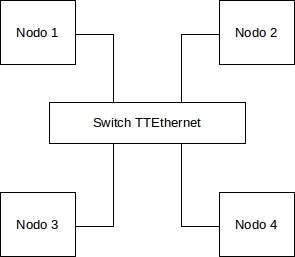
\includegraphics[scale=0.7]{images/Marco_teorico/TTEthernet_BUS.jpg}
  \caption{Arquitectura básica TTEthernet}
\label{fig:Arq_TTEthernet}
\end{figure}

TTEtheret puede actuar en dos clases de tráfico, con el objetivo de soportar diferentes niveles de cricticidad de mensajes. Estas clases de tráficos son las siguientes \citep{Loveless15} \citep{Steiner13}:
\begin{itemize}
	\item Time-Triggered, permite enviar mensajes de acuerdo a una planificación predefinida (scheduling),
	\item Rate-Constrained (RC), en el cual se llevan algunas restricciones de tamaño y rate de transmisión de frames,
	\item Best-Effort (BE), el cual se comporta de manera similar que el Ethernet
\end{itemize}

El paquete TTEthernet tiene una gran similitud con el frame del estándar IEEE 802.3 (Ethernet). Se denota en la Figura \ref{fig:Frame_TTEthernet} que en lugar de la MAC del 802.3 frame se divide en el CT Marker y el CTID. El primero es un identificador estático utilizado para distinguir paquetes \ac{TT} de otros tipos de tráficos.

\begin{figure}[h]
 \centering
 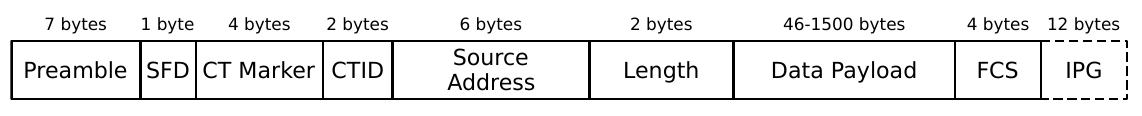
\includegraphics[scale=0.3]{images/Marco_teorico/Frame_TTEthernet.png}
  \caption{Frame de mensaje TTEthernet}
\label{fig:Frame_TTEthernet}
\end{figure}

El estándar SAE AS6802 define el protocolo de sincronización del TTEthernet. El protocolo TTP fue diseñado para reducir la complejidad de las arquitecturas distribuidas tolerantes a fallas \citep{TTTechWeb}. Existe un grupo de dispositivos de relojes locales que permite la sincronización requerida por la comunicación \ac{TT}, a esto se lo denomina \textif{dominio de sincronización} \citep{Loveless15}. Cada dominio de sincronización es asignado a uno de los siguientes roles:
\begin{itemize}
	\item Compression Master (CM)
	\item Synchronization Master (SM)
	\item Synchronization Cliente (SC)
\end{itemize}

\subsection{Experiencia de vuelo}
\cite{Loveless15} demuestra la aplicación de esta tecnología para computadoras de vuelo redundantes en misiones de naves simuladas. Esta tecnología toma tanto interés que el Sistema de Exploración Avanzada (AES)\footnote{Del ingles, Advanced Exploration Systems} de la \ac{NASA}, que lleva a cabo un proyecto denominado Avionics and Software (A&S). TTEthernet también fue utilizada en una arquitectura tolerante a fallas en el Integrated Power, Avionics and Software (IPAS)  del Johnson Space Center (JSC) y en el Core Flight Software (CFS) del Asteroid Redirect Mission (ARM) simulado\footnote{Los mencionados anteriormente son ejemplos de la utilización de TTEthernet} \citep{Loveless15}. También fue utilizado exitosamente durante la misión Orion \citep{TTTechOrion} .
TTEthernet simplifica el diseño de sistemas espaciales que deben contar con tolerancia a falla y una alta disponibilidad. La seguridad y la redundancia se mantiene sin ningún tipo de aplicación extra.
